\documentclass[a4paper,11pt]{article}

% ---------- Packages ----------
\usepackage[utf8]{inputenc}
\usepackage[T1]{fontenc}
\usepackage{graphicx}
\usepackage{amsmath}
\usepackage{amssymb}
\usepackage{siunitx}
\usepackage{geometry}
\usepackage{fancyhdr}
\usepackage{physics}
\usepackage{float}
\usepackage{caption}
\usepackage{subcaption}
\usepackage{hyperref}
\usepackage{xcolor}
\usepackage{subfiles} 
\usepackage{circuitikz}



% ---------- Page setup ----------
\geometry{margin=1.5cm}
\setlength{\parskip}{0.3em}
\setlength{\parindent}{0pt}

% ---------- Header/Footer ----------
\pagestyle{fancy}
\fancyhf{}
\lhead{DTU – Integrated Analog Electronics}
\rhead{Study No: s246132}
\cfoot{\thepage}

% ---------- Title ----------
\title{%
  \textbf{Integrated Analog Electronics – Assignment II}\\
  Exercises 1–6 (December 2025)
}
\author{Mads Rudolph \\ Study number: s246132}
\date{\today}

\begin{document}

\maketitle
\thispagestyle{empty}  

\begin{figure}
    \centering
    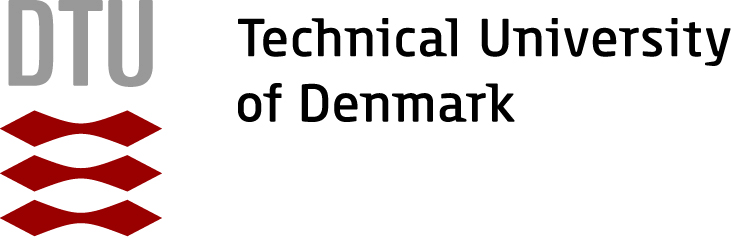
\includegraphics[width=0.3\linewidth]{images/DUT.png}
\end{figure}

\newpage
\tableofcontents
\newpage


\subfile{sections/exercise1_condensed}

\subfile{sections/exercise2_condensed}

\subfile{sections/exercise3_condensed}

\subfile{sections/exercise4_condensed}

\subfile{sections/exercise5_condensed}

\subfile{sections/exercise6_condensed}


\end{document}
